\section{Simulation Analysis}
\label{sec:simulation}

Before proceeding the theoretycal analysis, we simulated the circuit via the Ngspice software in order to perfect our parameters` values.

To simulate the transistor behaviour, we utilized the NPN and the PNP models provided by the professor.

We performed transient and frequency analysis of the combined gain and output stages, that represent, respectively, the common emitter and collector amplifiers.

\begin{figure}[h] \centering
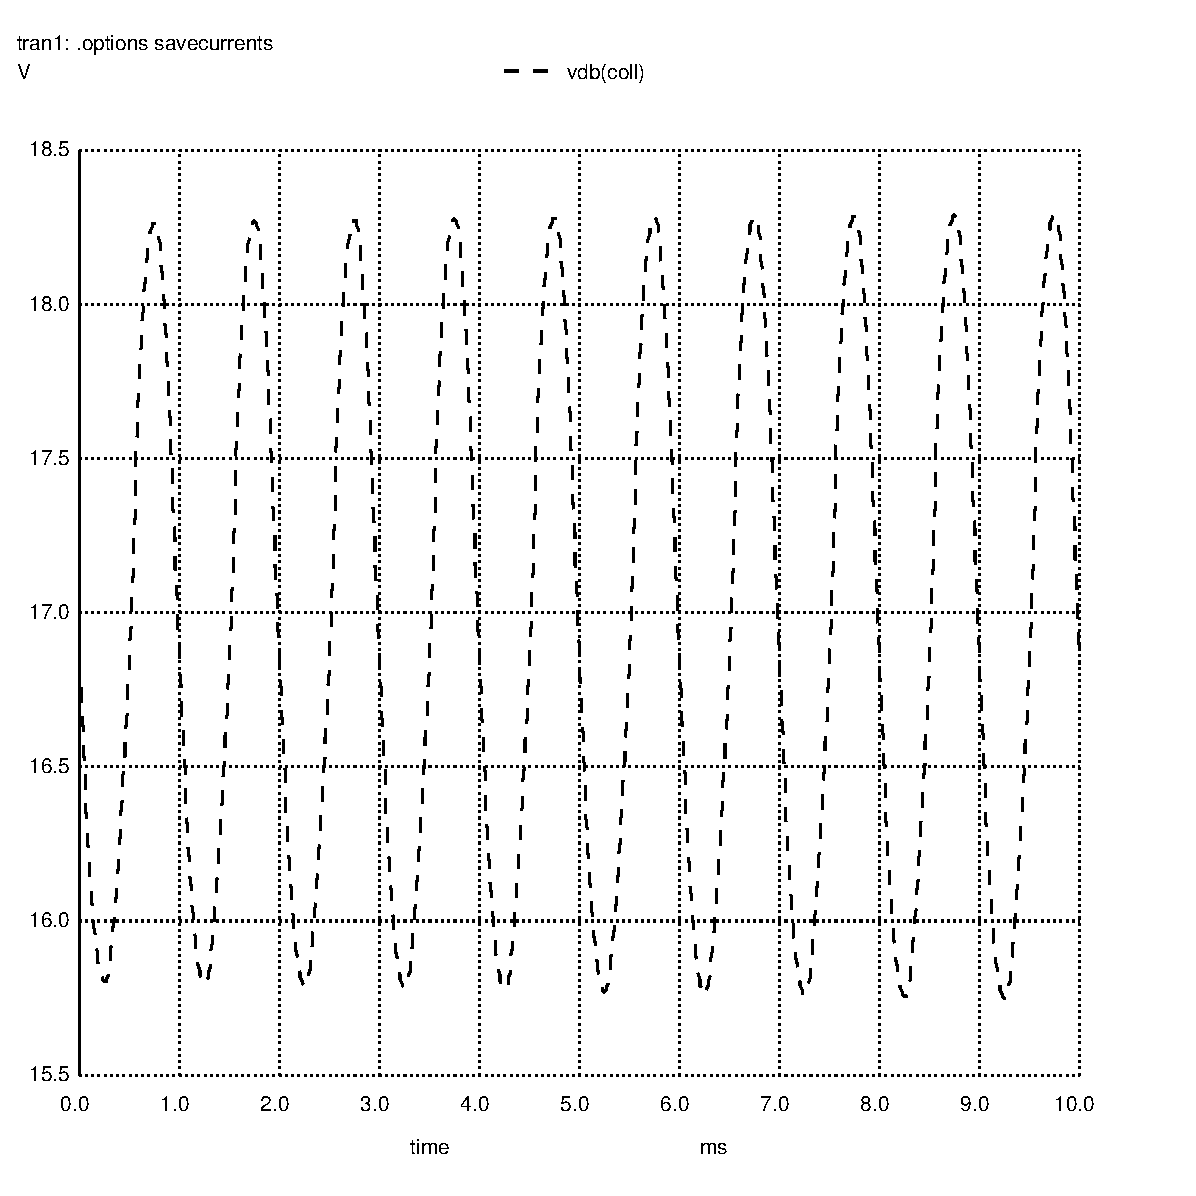
\includegraphics[width=0.6\linewidth]{vo1.eps}
\caption{Voltage in the collector, transient analysis.}
\label{fig:s1}
\end{figure}

\begin{figure}[h] \centering
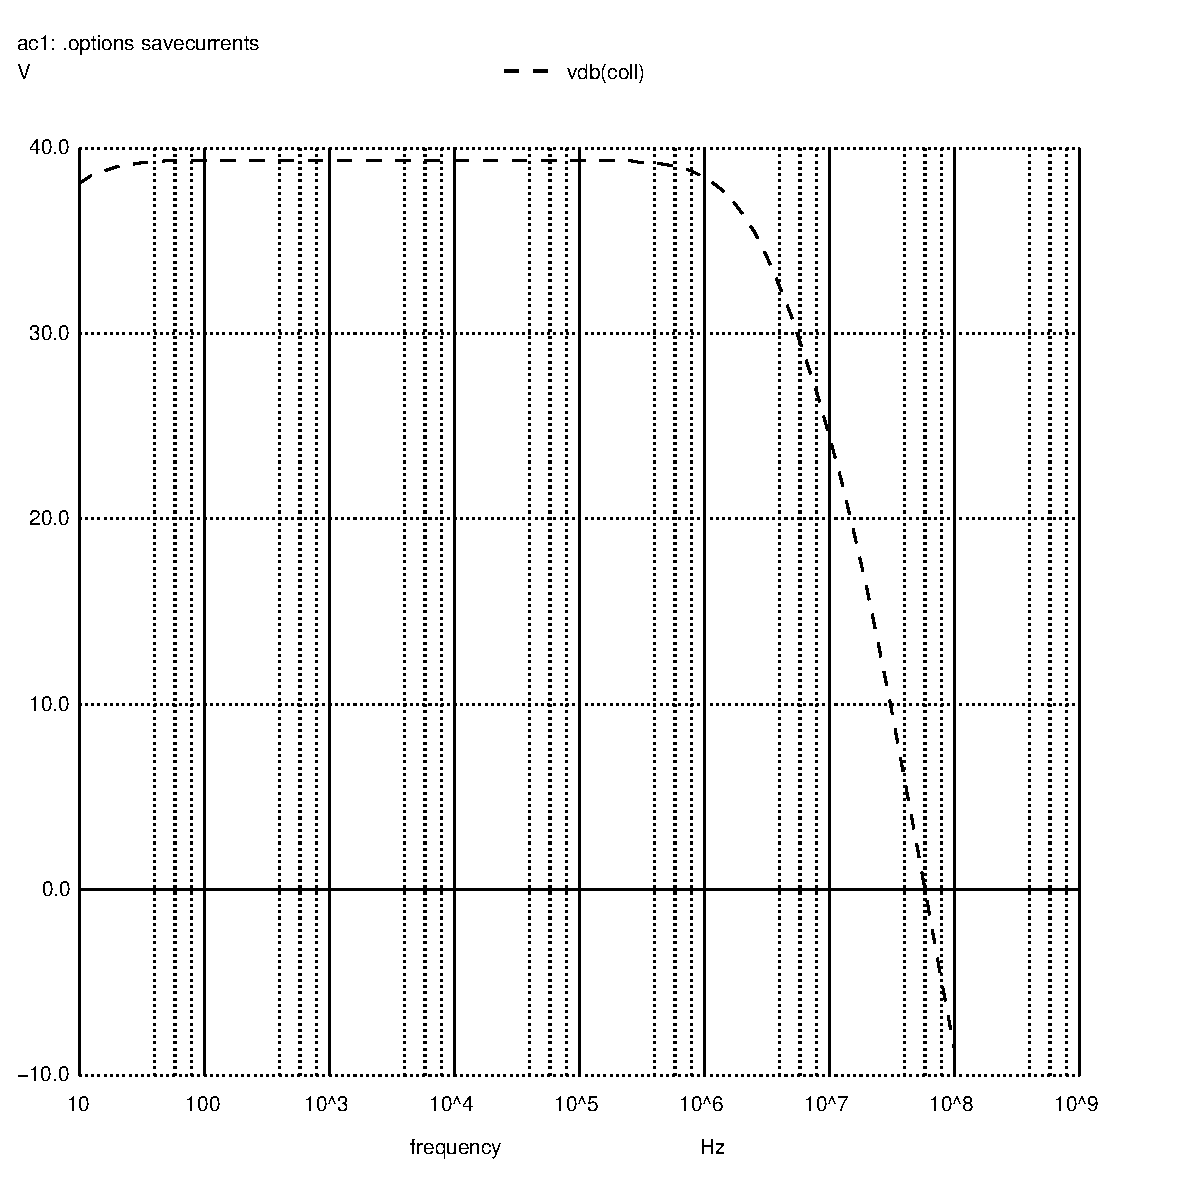
\includegraphics[width=0.6\linewidth]{vo1f.eps}
\caption{Voltage in the collector[dB], frequency analysis.}
\label{fig:s2}
\end{figure}

\begin{figure}[h] \centering
\includegraphics[width=0.6\linewidth]{vo3f.eps}
\caption{Phase voltage in the collector, frequency analysis.}
\label{fig:s3}
\end{figure}

\begin{figure}[h] \centering
\includegraphics[width=0.6\linewidth]{vo2f.eps}
\caption{Output voltage[dB].}
\label{fig:s4}
\end{figure}

\begin{figure}[h] \centering
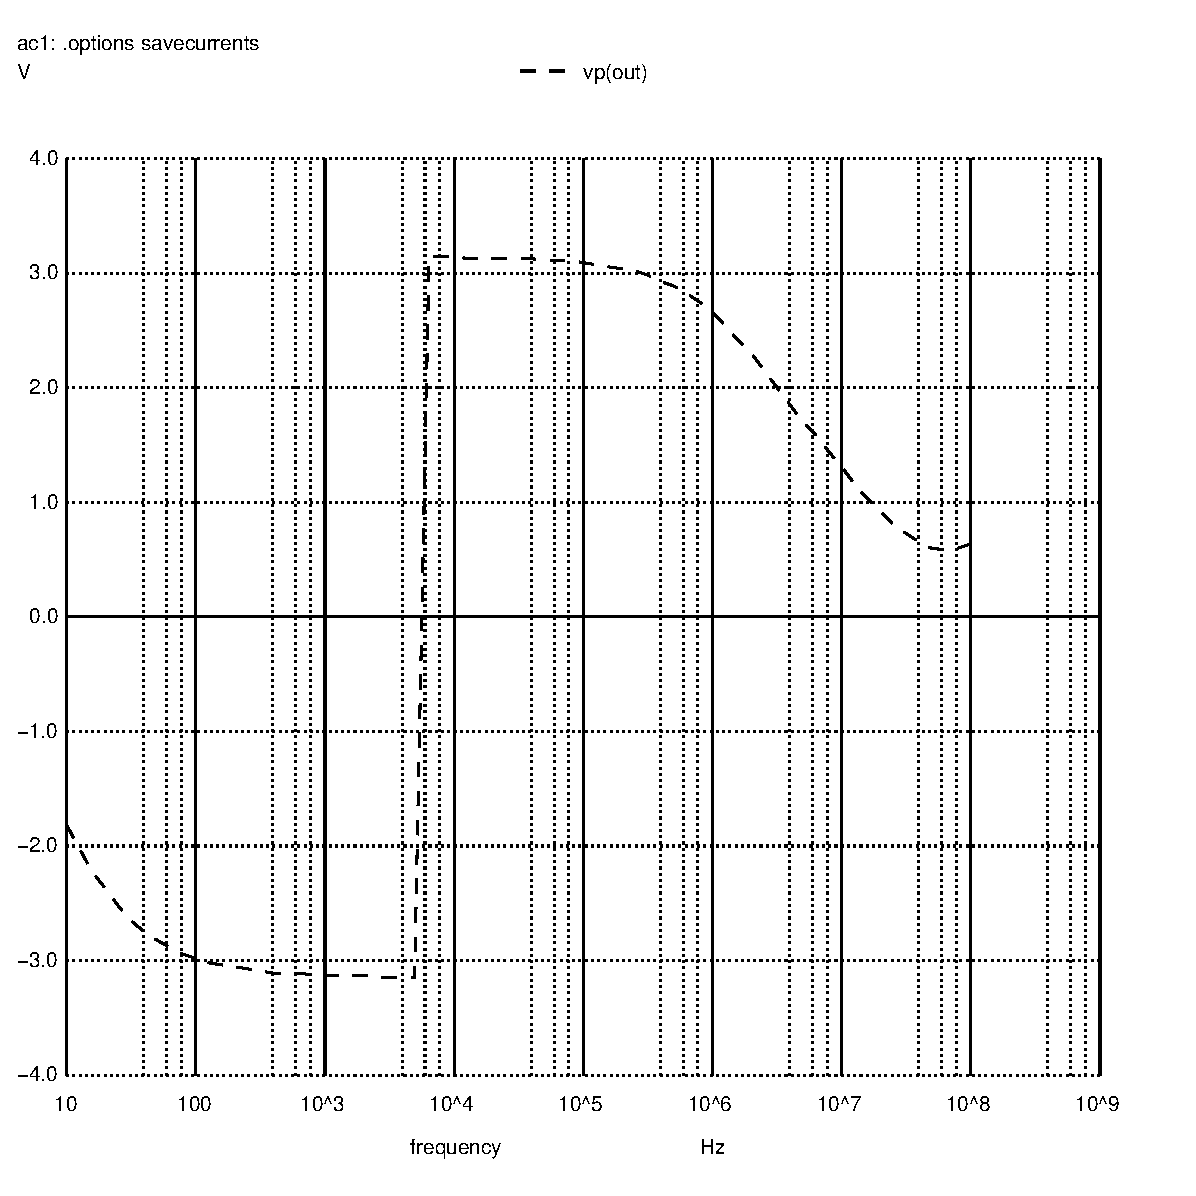
\includegraphics[width=0.6\linewidth]{vo4f.eps}
\caption{Output voltage phase.}
\label{fig:s5}
\end{figure}

From the simulation we were able to compute the important values of the cut-off frequencies, the gain and the bandwidth, which allowed us to calculate our merit. Furthermore, we found the values for the input and output impedances.

\begin{table}[h]
  \centering
  \begin{tabular}{|l|r|}
    \hline    
    {\bf Parameters} & {\bf Values} \\ \hline
    \input{op_TAB}
  \end{tabular}
  \caption{Values computed in the simulation.}
  \label{tab:s1}
\end{table}

\begin{table}[h]
  \centering
  \begin{tabular}{|l|r|}
    \hline    
    {\bf Parameters} & {\bf Values} \\ \hline
    \input{op_TAB2}
  \end{tabular}
  \caption{Output impedance.}
  \label{tab:s2}
\end{table}


